\chapter{Defining a new model}

Now that we know what a high-level job looks like, we can pick it apart and reduce the real-world measurements of one program to a more generic model. 

Summarizing the findings from the previous paragraphs; it was shown that 

\begin{itemize}
    \item The given job has phases that have different power draws
    \item Checkpointing \& resuming carries overhead in the form of startup costs and possible wasted work.
\end{itemize}

The parameters for the improved job model are shown in form of the python implementation in \ref{listing:model_python}. \todo{Check whether this ref works}

\todo{Probably need to improve the code here}
\begin{lstlisting}[language=python, frame=single, numbers=none, caption={Python Model definition}, basicstyle=\ttfamily, label={listing:model_python}]
class ModelParameters(TypedDict):
    startup: List[Phase]
    work: List[Phase]
    
class Phase(TypedDict):
    name: str
    duration: float
    power: float
    is_checkpoint: NotRequired[bool]   
\end{lstlisting}

Some simplifications are made: the duration of each phase is well known and the power per phase is a constant. 
Phases can also be named for later reference.
These phases essentially define a step function, i.e. piecewise constant function.
Unlike a traditional step function, the start- and endpoints of each "piece" would be encoded implicitly by the previous phases.
Using these specifications, a simple time-to-power function can be defined, that looks up the input time and traverses the phases in order.

Initially, I also considered allowing any expression instead of a constant value for power and then using Python's \verb|evaluate()| to e.g. allow a function-per-phase model.
In section \ref{sec:checkpoint_resume_lp}, having a rather restrictive step function will be of advantage, however. \todo{Add some more explanation to this in that section}

\todo[inline]{What to do if the events are not known? How does this work for more complex jobs}

The measurements that have been taken can now be fit into this new model. 
As each measurement-point can be associated to a phase via the aforementioned added logging, the average of each phase-associated measurement is used to determine the model parameters. 
The durations of the phases are calculated similarly by taking the average time the logging occurred during the measurements.

Using this strategy on the 10 complete runs results in figure \ref{fig:model_overlaid}, which shows the derived model on black with the previous figure \ref{fig:plot_full} in less opacity. 
The startup phase looks well approximated, visually however there is some error during the work phases.
The training phases each have a high variance, which is not captured by the constant power approximation. After each training  phase, the power goes down seemingly liniarly, which is also approxiimated by the constant.

One notable point, this model is a superset of the previous constant-no-overhead model used in the related work.
These jobs can be modeled with just one workphase, resulting in a constant power over its execution. Leaving the startup phases empty creates no overhead on resuming.

\todo{Should probably add the phase markers back in}
\begin{figure}
    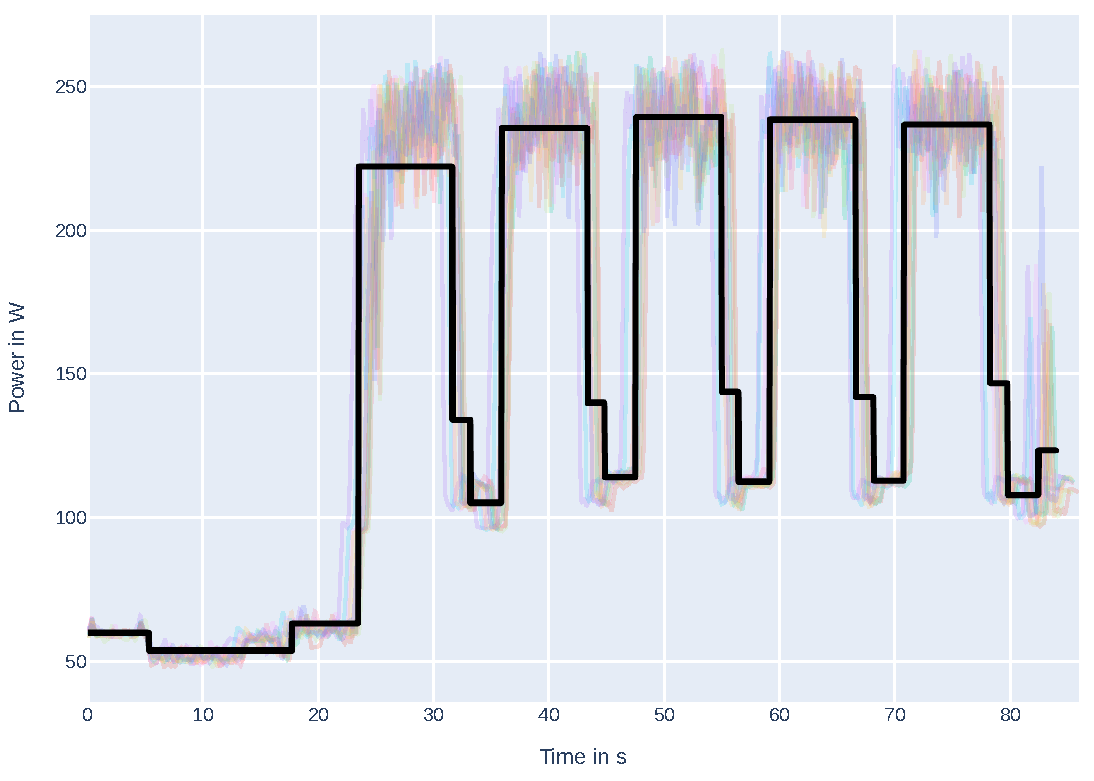
\includegraphics[width=\linewidth]{power-measurements/model_overlaid.pdf}
    \caption{Model of roberta.py (black) vs. all measurements}
    \label{fig:model_overlaid}
\end{figure}

\paragraph{Model error analysis}

To analyse the error of this model, I cross validated the power's and total energy's RMSE using \verb|scikit-learn|'s \verb|LeaveOneOut| strategy. 
The first one would give a measure of the model's accuracy on a short-time (sub-second) scale, the latter would  tell the long-time (whole job) scale accuracy of the model.

Each of the 10 runs would be taken as the ground truth while the other 9 would be used to create the model. The results are the following: t power between the prediction and remainder has an RSME of 39.3 W while the difference in total energy is calculated as -0.1 kJ. 

Interpreting this, it seems that the model performs poorly as a predictor for die exact power used at some timepoint as the RMSE is rather large (think of the maximum power drawn being about 250W). 
However, in the context of carbon aware scheduling, this should not be too big of an issue as the time frames for carbon-emissions are orders of magnitudes larger (electricitymaps has a resolution of 1 hour for each intenstiy of carbon emissions). 
The high error likely comes from the high variance during the training phases which is not captured in the model.

The total energy predicted by the model is very close to the actual real life experiment, this should mean that the total carbon calculated on the model should also be close to the carbon emitted by the real program.
